%
% $RCSfile: cybop.tex,v $
%
% Copyright (C) 2002-2008. Christian Heller.
%
% Permission is granted to copy, distribute and/or modify this document
% under the terms of the GNU Free Documentation License, Version 1.1 or
% any later version published by the Free Software Foundation; with no
% Invariant Sections, with no Front-Cover Texts and with no Back-Cover
% Texts. A copy of the license is included in the section entitled
% "GNU Free Documentation License".
%
% http://www.cybop.net
% - Cybernetics Oriented Programming -
%
% http://www.resmedicinae.org
% - Information in Medicine -
%
% Version: $Revision: 1.1 $ $Date: 2008-08-19 20:41:06 $ $Author: christian $
% Authors: Christian Heller <christian.heller@tuxtax.de>
%

%
% Determine document class specifying the type of document.
%
% Hand over font size and side format.
%
\documentclass[9pt,twoside]{tuxtax}

%
% Input hyphenation list.
%
%%
% $RCSfile: hyphenation.tex,v $
%
% Copyright (c) 2001-2004. Christian Heller. All rights reserved.
%
% No copying, altering, distribution or any other actions concerning this
% document, except after explicit permission by the author!
% At some later point in time, this document is planned to be put under
% the GNU FDL license. For now, _everything_ is _restricted_ by the author.
%
% http://www.cybop.net
% - Cybernetics Oriented Programming -
%
% http://www.resmedicinae.org
% - Information in Medicine -
%
% @author Christian Heller <christian.heller@tuxtax.de>
%

\hyphenation{abs-trac-tion}
\hyphenation{abs-trac-tions}
\hyphenation{ac-tu-ally}
\hyphenation{addi-tio-nally}
\hyphenation{ana-lyst}
\hyphenation{ana-ly-sis}
\hyphenation{an-cient}
\hyphenation{ap-pli-ca-tion}
\hyphenation{arche-types}
\hyphenation{aris-to-tle}
\hyphenation{at-tri-bute}
\hyphenation{avoi-da-ble}
\hyphenation{be-ing}
\hyphenation{binary}
\hyphenation{bran-ches}
\hyphenation{ca-te-go-ri-za-tion}
\hyphenation{client}
\hyphenation{com-po-nen-ti-za-tion}
\hyphenation{com-pu-ter}
\hyphenation{con-fi-gure}
\hyphenation{con-fi-gu-ra-tion}
\hyphenation{con-nec-ted}
\hyphenation{cri-ti-cised}
\hyphenation{cy-ber-ne-tics}
\hyphenation{cyboi}
\hyphenation{cybol}
\hyphenation{cybop}
\hyphenation{de-sign}
\hyphenation{des-cribe}
\hyphenation{des-cribed}
\hyphenation{de-ve-lop-ment}
\hyphenation{dis-crete}
\hyphenation{di-vide}
\hyphenation{do-main}
\hyphenation{dy-na-mic}
\hyphenation{dy-na-mics}
\hyphenation{ela-bo-ra-ted}
\hyphenation{ele-ments}
\hyphenation{en-gi-nee-ring}
\hyphenation{eng-lish}
\hyphenation{en-vi-ron-ment}
\hyphenation{ex-pert}
\hyphenation{fi-gure}
\hyphenation{fun-da-men-tal}
\hyphenation{func-tio-na-li-ty}
\hyphenation{hard-ware}
\hyphenation{hu-man}
\hyphenation{im-ple-men-ta-tion}
\hyphenation{imp-roved}
\hyphenation{in-he-rit}
\hyphenation{in-ter-pre-ter}
\hyphenation{java}
\hyphenation{know-ledge}
\hyphenation{lan-guage}
\hyphenation{li-ving}
\hyphenation{lo-gi-cal}
\hyphenation{machine}
\hyphenation{me-cha-nism}
\hyphenation{me-thods}
\hyphenation{na-ture}
\hyphenation{net-work}
\hyphenation{neu-ral}
\hyphenation{neu-ron}
\hyphenation{nu-me-rous}
\hyphenation{object}
\hyphenation{open}
\hyphenation{operating}
\hyphenation{ori-en-ted}
\hyphenation{over-come}
\hyphenation{prin-ci-ple}
\hyphenation{prin-ting}
\hyphenation{pro-ba-bi-lis-tic}
\hyphenation{pro-gram-ming}
\hyphenation{re-cog-nize}
\hyphenation{re-cog-nized}
\hyphenation{re-pre-sen-ta-tion}
\hyphenation{re-pre-sen-ting}
\hyphenation{re-u-sa-bi-li-ty}
\hyphenation{sci-ence}
\hyphenation{server}
\hyphenation{se-pa-ra-ted}
\hyphenation{se-pa-ra-tion}
\hyphenation{si-mi-lar}
\hyphenation{soft-ware}
\hyphenation{source}
\hyphenation{spe-cia-li-za-tion}
\hyphenation{sta-tic}
\hyphenation{sta-ti-cal-ly}
\hyphenation{sto-chas-tic}
\hyphenation{stone-on-stone}
\hyphenation{struc-ture}
\hyphenation{strug-gling}
\hyphenation{su-per-flu-ous}
\hyphenation{sup-ply-ing}
\hyphenation{sys-tem}
\hyphenation{tes-ting}
\hyphenation{thin-king}
\hyphenation{un-en-li-vened}
\hyphenation{un-fa-vou-ra-ble}
\hyphenation{un-sa-tis-fy-ing}
\hyphenation{va-ry-ing}
\hyphenation{weigh-ted}


%
% Define text macros.
%
\def\placemacro{Ilmenau}
\def\datemacro{2005-12-12}
\def\authormacro{Christian Heller}

%
% Enable special indexing commands.
% Generate contents, glossary and memo entries.
%
% Required package: makeidx
%
\makeindex

%
% This document arose from the dissertation of Christian Heller,
% written to earn a doctorate in Software Systems Engineering.
%
% Author: Christian Heller <christian.heller@tuxtax.de>
%
\begin{document}
    % Set sans serif font.
    \sffamily
    % Set page numbering to roman numbers.
    \pagenumbering{roman}
    %
% $RCSfile: cover.tex,v $
%
% Copyright (C) 2002-2008. Christian Heller.
%
% Permission is granted to copy, distribute and/or modify this document
% under the terms of the GNU Free Documentation License, Version 1.1 or
% any later version published by the Free Software Foundation; with no
% Invariant Sections, with no Front-Cover Texts and with no Back-Cover
% Texts. A copy of the license is included in the section entitled
% "GNU Free Documentation License".
%
% http://www.cybop.net
% - Cybernetics Oriented Programming -
%
% http://www.resmedicinae.org
% - Information in Medicine -
%
% Version: $Revision: 1.1 $ $Date: 2008-08-19 20:41:06 $ $Author: christian $
% Authors: Christian Heller <christian.heller@tuxtax.de>
%

%
% Defines the title page.
%
% \title and \author (and optionally \date) must be specified!
%
% Sets the page style of the first page to empty
% that is no header or footer will be shown.
%
\begin{titlepage}
    \title{
        Cybernetics Oriented Programming\\
        (CYBOP)\\
        \vspace{1cm}
        % \textmd sets medium weight (default), which is the opposite of boldface.
        \normalsize{\textmd{An Investigation on the Applicability of Inter-Disciplinary Concepts\\
            to Software System Development\\}}
    }
    \author{
        \date{
        }
    }
\end{titlepage}

    \maketitle
    % Avoid header, footer and page number.
    \thispagestyle{empty}
    %
% $RCSfile: title.tex,v $
%
% Copyright (c) 2001-2004. Christian Heller. All rights reserved.
%
% No copying, altering, distribution or any other actions concerning this
% document, except after explicit permission by the author!
% At some later point in time, this document is planned to be put under
% the GNU FDL license. For now, _everything_ is _restricted_ by the author.
%
% http://www.cybop.net
% - Cybernetics Oriented Programming -
%
% http://www.resmedicinae.org
% - Information in Medicine -
%
% @author Christian Heller <christian.heller@tuxtax.de>
%

\title{A new Pattern Systematics}
\author{
    Christian Heller \(<\)christian.heller@tu-ilmenau.de\(>\)\\
    Detlef Streitferdt \(<\)detlef.streitferdt@tu-ilmenau.de\(>\)\\
    Ilka Philippow \(<\)ilka.philippow@tu-ilmenau.de\(>\)
}
\institute{Technical University of Ilmenau\\
    Faculty for Computer Science and Automation\\
    Institute for Theoretical and Technical Informatics\\
    PF 100565, Max-Planck-Ring 14, 98693 Ilmenau, Germany\\
    http://www.tu-ilmenau.de, fon: +49-3677-69-1230, fax: +49-3677-69-1220 \vspace*{0.5cm}
}

    \newpage{\pagestyle{empty}\clearpage}
    \thispagestyle{empty}
    %
% $RCSfile: copyright.tex,v $
%
% Copyright (c) 2002-2007. Christian Heller. All rights reserved.
%
% Permission is granted to copy, distribute and/or modify this document
% under the terms of the GNU Free Documentation License, Version 1.1 or
% any later version published by the Free Software Foundation; with no
% Invariant Sections, with no Front-Cover Texts and with no Back-Cover
% Texts. A copy of the license is included in the section entitled
% "GNU Free Documentation License".
%
% http://www.cybop.net
% - Cybernetics Oriented Programming -
%
% Version: $Revision: 1.2 $ $Date: 2007-08-01 13:59:00 $ $Author: christian $
% Authors: Christian Heller <christian.heller@tuxtax.de>
%

\small{Cataloging-in-Publication Data\\\\
    \authormacro.\\
    \titlemacro:\\
    \subtitlemacro\\
    \versionmacro\\
    \placemacro: Tux Tax, 2007%\\
%    ISBN-10: 3-9810898-0-4 xxx EDIT xxx\\
%    ISBN-13: 978-3-9810898-0-6 xxx EDIT xxx
}\\

\small{Information about this specification\\
    http://www.cybop.net, http://www.tuxtax.de}

\vspace{4cm}

\small{Copyright \textcopyright\ 2002-2007. \authormacro. All rights reserved.}

%> \small{Translation: Christian Heller}\\ %\"Ubersetzung:
%\small{Sponsoring Editor: ??}\\ %Lektorat:
%\small{Acquisitions Editor: ??}\\
%\small{Marketing Manager: ??}\\
%\small{Marketing Assistant: ??}\\
%\small{Editorial Assistant: ??}\\
%\small{Editorial/ Production Supervision: ??}\\
%\small{Production Editor: Christian Heller}\\ %Produktion:
%\small{Production Service: ??}\\ %Produktion:
%\small{Manuscript Editor: ??}\\
%\small{Interior Illustration: ??}\\
%\small{Interior Design: ??}\\
%\small{Cover Illustration: TSAMEDIEN, D\"usseldorf}\\ %Umschlaggrafik:
%\small{Cover Design: Christian Heller}\\ %Umschlaggestaltung:
%\small{Print Buyer: ??}\\
%\small{Project Coordinator: ??}\\
%> \small{Typesetting: Christian Heller, set in Times 9.5 pt font with \LaTeX\ using Kile under Linux}\\ %Satz:
%\small{Cover Printing: ??}\\
%\small{Printing and Binding: Offizin Andersen Nex\"o, Leipzig/ Zwenkau} %Belichtung, Druck und Bindung:

\small{Permission is granted to copy, distribute and/or modify this document
    under the terms of the GNU Free Documentation License, Version 1.2
    or any later version published by the Free Software Foundation;
    with no Invariant Sections, with no Front-Cover Texts and with no
    Back-Cover Texts. A copy of the license is included in the section
    entitled "GNU Free Documentation License".}

\small{Trademark Credits\\
    Most of the software-, hardware- and product names used in this document
    are also trademarks or registered trademarks of their respective owners.
%    Adobe is a trademark of Adobe Systems, Incorporated.\\
%    AIX is a trademark of International Business Machines Corporation.\\
%    Arial\textregistered\ is a registered trademark of the Monotype Corporation in the United States and other countries.\\
%>    CICS is a trademark of International Business Machines Corporation.\\
%    CICS/ESA is a trademark of International Business Machines Corporation.\\
%    CorelDRAW\texttrademark\ is a trademark or registered trademark of Corel Corporation or Corel Corporation Limited.\\
%>    DB2 is a trademark of International Business Machines Corporation.\\
%    DFSMS is a trademark of International Business Machines Corporation.\\
%    DFSORT is a trademark of International Business Machines Corporation.\\
%    Energy Star\textregistered\ and the Energy Star logo\textregistered\ are registered marks of the United States Environmental Protection Agency in the United States and other countries. Details on the proper use of the marks are explained in the "Guidelines for Proper use of the Energy Star\textregistered\ Name and International Logo".\\
%>    Ethernet is a registered trademark of Xerox Corporation.\\
%>    IBM\textregistered\ is a registered trademark of International Business Machines Corporation.\\
%    IBM Warp Server\textregistered\ is a registered trademark of International Business Machines Corporation.\\
%    IMS is a trademark of International Business Machines Corporation.\\
%    IMS/ESA is a trademark of International Business Machines Corporation.\\
%>    Intel is a registered trademark of Intel Corporation in the United States and other countries.\\
%>    Java\texttrademark\ and all Java-based trademarks are trademarks of Sun Microsystems, Inc. in the United States and other countries.\\
%    Language Environment is a trademark of International Business Machines Corporation.\\
%>    Microsoft\textregistered\ is a registered trademark of Microsoft Corporation in the United States and other countries.\\
%    MS Windows\textregistered\ is a registered trademark of Microsoft Corporation in the United States and other countries.\\
%    MS-DOS\textregistered\ is a registered trademark of Microsoft Corporation in the United States and other countries.\\
%    MVS is a trademark of International Business Machines Corporation.\\
%    Netscape is a trademark of Netscape Communications Corporation in the United States and other countries.\\
%    Netscape Navigator is a trademark of Netscape Communications Corporation in the United States and other countries.\\
%    Netware\textregistered\ is a registered trademark of Novell Corporation.\\
%    Novell\textregistered\ is a registered trademark of Novell Corporation.\\
%    OpenEdition is a trademark of International Business Machines Corporation.\\
%    Opera\texttrademark\ is a trademark of Opera Software ASA.\\
%    Operating System/2\textregistered\ (OS/2) is a registered trademark of International Business Machines Corporation.\\
%    *Pantone, Inc. is a check-standard trademark for color.\\
%>    Pentium is a registered trademark of Intel Corporation in the United States and other countries.\\
%>    PostScript is a trademark of Adobe Systems, Incorporated.\\
%    RACF is a trademark of International Business Machines Corporation.\\
%    System/390 is a trademark of International Business Machines Corporation.\\
%>    Unicode is a trademark of the Unicode Consortium.\\
%>    UNIX\textregistered\ is a registered trademark of The Open Group in the United States and other countries.\\
%    VisualAge is a trademark of International Business Machines Corporation.\\
%>    Windows\textregistered\ is a registered trademark of Microsoft Corporation in the United States and other countries.\\
%    Windows NT\textregistered\ is a registered trademark of Microsoft Corporation in the United States and other countries.\\
%    z/OS is a trademark of International Business Machines Corporation.\\
%>    Other company-, product- or service names may be the trademarks or service marks of others.\\
}

\small{Donations\\
    Companies using CYBOP ideas, CYBOL or CYBOI on a grand scale are asked to
    notify the author \(<\)christian.heller@tuxtax.de\(>\) and to consider
    donating some of their sales revenues, which will be used exclusively for
    the CYBOP and Res Medicinae free software projects.}

%\small{Text printed on recycled and acid-free paper.}

\small{Made in Germany, Europe, Planet Earth}

    \newpage{\pagestyle{empty}\cleardoublepage}
    % Avoid header, footer and page number.
    \thispagestyle{empty}
    %
% $RCSfile: dedication.tex,v $
%
% Copyright (C) 2002-2008. Christian Heller.
%
% Permission is granted to copy, distribute and/or modify this document
% under the terms of the GNU Free Documentation License, Version 1.1 or
% any later version published by the Free Software Foundation; with no
% Invariant Sections, with no Front-Cover Texts and with no Back-Cover
% Texts. A copy of the license is included in the section entitled
% "GNU Free Documentation License".
%
% http://www.cybop.net
% - Cybernetics Oriented Programming -
%
% http://www.resmedicinae.org
% - Information in Medicine -
%
% Version: $Revision: 1.1 $ $Date: 2008-08-19 20:41:06 $ $Author: christian $
% Authors: Christian Heller <christian.heller@tuxtax.de>
%

\vspace*{3cm}
\begin{center}
    To all kind-hearted People who contribute to Humanity;\\
    against Those whose only Aim in Life is to amass Money
\end{center}

    \newpage{\pagestyle{empty}\cleardoublepage}
    \tableofcontents
    \newpage{\pagestyle{empty}\cleardoublepage}
    % Set roman font.
    \rmfamily
    %
% $RCSfile: preface.tex,v $
%
% Copyright (C) 2002-2008. Christian Heller.
%
% Permission is granted to copy, distribute and/or modify this document
% under the terms of the GNU Free Documentation License, Version 1.1 or
% any later version published by the Free Software Foundation; with no
% Invariant Sections, with no Front-Cover Texts and with no Back-Cover
% Texts. A copy of the license is included in the section entitled
% "GNU Free Documentation License".
%
% http://www.cybop.net
% - Cybernetics Oriented Programming -
%
% http://www.resmedicinae.org
% - Information in Medicine -
%
% Version: $Revision: 1.1 $ $Date: 2008-08-19 20:41:08 $ $Author: christian $
% Authors: Christian Heller <christian.heller@tuxtax.de>
%

\chapter*{Preface\markboth{Preface}{Preface}}
\label{preface_heading}
\addcontentsline{toc}{chapter}{Preface}

\begin{flushright}
    \textsl{
        I slept and dreamt that Life was Joy.\\
        I awoke and saw that Life was Service.\\
        I acted and behold, Service was joy.
    }\\
    \textsc{Rabindranath Tagore}
\end{flushright}

%
% $RCSfile: prologue.tex,v $
%
% Copyright (C) 2002-2008. Christian Heller.
%
% Permission is granted to copy, distribute and/or modify this document
% under the terms of the GNU Free Documentation License, Version 1.1 or
% any later version published by the Free Software Foundation; with no
% Invariant Sections, with no Front-Cover Texts and with no Back-Cover
% Texts. A copy of the license is included in the section entitled
% "GNU Free Documentation License".
%
% http://www.cybop.net
% - Cybernetics Oriented Programming -
%
% http://www.resmedicinae.org
% - Information in Medicine -
%
% Version: $Revision: 1.2 $ $Date: 2008-09-07 15:36:07 $ $Author: christian $
% Authors: Christian Heller <christian.heller@tuxtax.de>
%

\section*{Prologue}
\label{prologue_heading}
%\addcontentsline{toc}{section}{Prologue}

To me, basically, there are two ways to deal with a scientific subject:

\begin{enumerate}
    \item The deepened investigation on a special area aiming to find
        completely new phenomenons
    \item The systematic subsumption of multiple known aspects of one or many
        disciplines aiming to find new cross-correlations and ideas
\end{enumerate}

Both approaches may lead to new theories, methods and concepts. And both may use
laboratory trials to find and prove their theories. This work follows the second
approach. The idea behind is, simply spoken, to steal ideas from nature and
various fields of science, and to apply them to software design.

\emph{Laboratory Trials} are what \emph{Coding} is in informatics -- experiment
and proof of operability, at the same time. Some information scientists have
the opinion that coding weren't \emph{scientific} enough and not necessary to
create new theories or to achieve good results. I doubt this. In my opinion,
there are things that can only be found when actually implementing ideas in a
computer language. And in the end, a theory is worth much more when having been
proven in practice. This document contains proven ideas that were growing in my
mind over the last few years, while dealing with topics such as:

\begin{itemize}
    \item[-] Structured- and Procedural Programming
    \item[-] Object Oriented Programming
    \item[-] Design Patterns and Frameworks
    \item[-] Component Based Design and Agents
    \item[-] Ontology Structured Domain Knowledge
    \item[-] Document- and User Interface Markup
    \item[-] Persistence Mechanisms
    \item[-] System Communication
    \item[-] Operating System Concepts
\end{itemize}

The usage of typical buzzwords could not quite be avoided in this work, yet do
I hope that the ideas and results are nevertheless explained straightforward and
well enough to be really useful to some other developers out there.

This document claims to be an \emph{Academic Paper}. To all practitioners who do
not want to read it for that reason, I would like to point out that each and
every concept in it arose from practice, that is coding. Like most developers,
I started up with only a few lines of code in one Java class, later extended to
more classes, a whole framework and so on. Whenever I stumbled over difficulties,
I thought through and improved my current design by applying patterns recommended
by several software development Gurus. It was only when I realised that even
those concepts were not sufficient, that I made up my own. They are entitled
\emph{Cybernetics Oriented Programming} (CYBOP), because most ideas behind them
stem from nature.

Finally, this document has become my thesis, written to earn a doctorate
(Dr.-Ing./ PhD) in Informatics/ Software Engineering. You may wonder why I
release it under the \emph{Free Documentation License} (FDL). Well, I'm a full
supporter of the idea of \emph{Free Knowledge}, \emph{Free Software}, a
\emph{Society free of Patents} which are only hindering its development. There
are three reasons that have contributed to my decision:

\begin{enumerate}
    \item Hope to get helpful \emph{Feedback} from readers
    \item Trust in the scientific \emph{Fairness} of colleagues, worldwide, to
        properly reference this document even though it is licensed under the FDL
    \item Wish to contribute to the open source movement \emph{now} (and not in
        some years when the document might reach a more stable version), to
        speed up its successful development
\end{enumerate}

This is a growing document undergoing steady development. It is not and doesn't
claim to be free of errors nor to contain the only possible way for application
system development. So, if you find errors of whatever kind or have any helpful
ideas or constructive criticism, then please contribute them to
\(<\)christian.heller@tuxtax.de\(>\) or to the CYBOP developers mailing list
\(<\)cybop-developers@lists.berlios.de\(>\)!

%
% $RCSfile: scientific_progress.tex,v $
%
% Copyright (C) 2002-2008. Christian Heller.
%
% Permission is granted to copy, distribute and/or modify this document
% under the terms of the GNU Free Documentation License, Version 1.1 or
% any later version published by the Free Software Foundation; with no
% Invariant Sections, with no Front-Cover Texts and with no Back-Cover
% Texts. A copy of the license is included in the section entitled
% "GNU Free Documentation License".
%
% http://www.cybop.net
% - Cybernetics Oriented Programming -
%
% http://www.resmedicinae.org
% - Information in Medicine -
%
% Version: $Revision: 1.1 $ $Date: 2008-08-19 20:41:08 $ $Author: christian $
% Authors: Christian Heller <christian.heller@tuxtax.de>
%

\section*{Scientific Progress}
\label{scientific_progress_heading}
%\addcontentsline{toc}{section}{Scientific Progress}

An \emph{Abstraction} allows to capture the real world by representing it in
simplified models. Such models contain only the essential aspects of a special
domain. Any unimportant nuances, in the considered context, are neglected.
Correct abstract models is what makes science easy. Good science \emph{can} be
\emph{easy}. If it is not, then probably either:

\begin{itemize}
    \item[-] there is a \emph{mistake} in the model
    \item[-] it is not fully \emph{understood} by the scientist him/ herself
    \item[-] the explaining person wants to \emph{keep back} knowledge, making
        others look clueless
\end{itemize}

One of the biggest hindrances to scientific progress is too much or false
respect for existing solutions. No theory/ model/ concept is ever finished;
no document/ software/ product is ever fully completed. There is always room
for improvements. In the end, it is all just a person's subjective perception
and an arbitrary, abstract extract of the real world.

It is always worth reviewing and questionning everything in depth, again and
again. Standstill means regress. The best example showing how to work around
these criticisms is the \emph{Free and Open Source Software} (FOSS) movement
where all the time, existing solutions are rewritten, to be improved.

%
% $RCSfile: software_patents.tex,v $
%
% Copyright (C) 2002-2008. Christian Heller.
%
% Permission is granted to copy, distribute and/or modify this document
% under the terms of the GNU Free Documentation License, Version 1.1 or
% any later version published by the Free Software Foundation; with no
% Invariant Sections, with no Front-Cover Texts and with no Back-Cover
% Texts. A copy of the license is included in the section entitled
% "GNU Free Documentation License".
%
% http://www.cybop.net
% - Cybernetics Oriented Programming -
%
% http://www.resmedicinae.org
% - Information in Medicine -
%
% Version: $Revision: 1.1 $ $Date: 2008-08-19 20:41:08 $ $Author: christian $
% Authors: Christian Heller <christian.heller@tuxtax.de>
%

\section*{Software Patents}
\label{software_patents_heading}
%\addcontentsline{toc}{section}{Software Patents}

This work is about software. Software abstracts the real world, its items and
processes, and it can store these information and their relations which make up
actual \emph{Knowledge}. In the modern, so-called \emph{Information Society},
it becomes more and more important to have \emph{free} access to external
knowledge. This is an \emph{essential} human right and will decide about the
future living quality of people.

So much the important it is to \emph{prohibit} the application of patents to
software! They make an exclusive club of large companies own the rights on
banal, ordinary, day-to-day algorithms and methods that many people use. And,
they thereby kill any new ideas and hinder research efforts that depend on
these basic algorithms. If \emph{Software Patents} and patents on
\emph{Computer Implemented Inventions} (CII) got introduced, any free software
developer and especially \emph{Small- and Medium Sized Enterprises} (SME), the
driving force of innovation, could not unfold their full potential anymore,
since much of their time and effort would then have to go into patent inquiries
and costly legal disputes.

Software patents are dangerous for the free development of thoughts! Certain
lobbies exert an increasing influence on politics and push members of
parliaments to agitate and vote in their interest. Since probably every reader
of this document has an interest in informatics, every reader is also affected
by the software patent enforcement. But everybody can do something about it,
not only in Europe! Express your protest and sign the petition at \cite{ffii}!

%
% $RCSfile: free_publishing.tex,v $
%
% Copyright (C) 2002-2008. Christian Heller.
%
% Permission is granted to copy, distribute and/or modify this document
% under the terms of the GNU Free Documentation License, Version 1.1 or
% any later version published by the Free Software Foundation; with no
% Invariant Sections, with no Front-Cover Texts and with no Back-Cover
% Texts. A copy of the license is included in the section entitled
% "GNU Free Documentation License".
%
% http://www.cybop.net
% - Cybernetics Oriented Programming -
%
% http://www.resmedicinae.org
% - Information in Medicine -
%
% Version: $Revision: 1.1 $ $Date: 2008-08-19 20:41:06 $ $Author: christian $
% Authors: Christian Heller <christian.heller@tuxtax.de>
%

\section*{Free Publishing}
\label{free_publishing_heading}
%\addcontentsline{toc}{section}{Free Publishing}

Reputation in the scientific world strongly depends on the number of
publications in scientific journals, conference proceedings, magazines etc., of
which some have greater kudos, some less. A \emph{Philosophiae Doctor} (PhD)
student, for example, is expected to publish in some of the \emph{acknowledged}
journals, in order to be conferred a doctorate. The grant of project fundings
by local-, national- or \emph{European Union} (EU) governements and sponsorship
of a professor's department at university depend on it as well. Some unfair
practices and shortcomings of the current system of publication shall therefore
be mentioned here. There are at least four disadvantages of publishing in
scientific journals. An author:

\begin{itemize}
    \item is almost always forced to assign his copyright to the publisher;
    \item has very little chance of publishing completely new ideas, since
        evaluators (which are to guarantee a certain \emph{scientific level})
        sieve those which seem too crazy or are unknown to them and do not
        match state-of-the-art science, so that really new ideas can hardly
        become popular in this way;
    \item has to wait many months before being informed about article
        acceptance, sometimes further months to presentation at a conference
        and yet more months until a journal/ proceedings are finally available
        -- which, besides the unfine delay, is enough time for an evaluator to
        adapt the best ideas and publish them in a modified form before;
    \item and everyone else have to pay money for receiving journals (even for
        the one containing the author's own work), or become a member of
        certain scientific societies for some discount -- which means that the
        work is not freely accessible.
\end{itemize}

Further, there is something often labelled \emph{Citation Mafia}. Whether an
article gets published in a journal or not depends on it being accepted by a
number of reviewers (normally three). In order to avoid personal battles, the
article author never gets to know the evaluators' names or proficiency and has
to blindly rely on the \emph{good taste} of a conference's program committee.
However, evaluators, although tied to ethical standards, often seem to have
their list of \emph{friends} or seem to just prefer authors who have already
published elsewhere, leading to circles of scientists citing each other, quite
independent from the quality of their papers. Logically, also here, there are a
number of disadvantages:

\begin{itemize}
    \item Young scientists have a hard life and need a long time for getting
        their articles accepted, independent from how innovative they are.
    \item Mafioso scientists often warm up old stories or deliver well-formulated,
        but rubbish articles not earning the predicate \emph{scientific}.
\end{itemize}

Don't ask for proof -- I don't have it. But almost everybody in the scientific
business knows about these issues. Unfortunately, only few people \cite{jobb}
talk about- or try to change them. Obviously, many scientists prefer to either
play the same old game or are scared of personal disadvantages. However, it
feels like increasingly more researchers, in particular the new generation,
become aware that these drawbacks hinder scientific progress and new solutions
need to be found. Well, there is free online journals such as the
\emph{Journal of Free and Open Source Medical Computing} (JOSMC) \cite{josmc}
or the \emph{BioMed Central} (BMC) \cite{bmc} publisher, where research
articles are: \textit{free to access immediately, peer reviewed,
citation-tracked \ldots}

Although this document cannot deliver solutions to the above-mentioned
problems, it mentioned those to inform the reader and spur further discussion.
Supportive actions in this process would be that:

\begin{itemize}
    \item scientists acknowledge no-cost entry open source conferences like
        LinuxTag \& Co. \cite{linuxtag} as alternatives to traditional ones
    \item professors more readily accept citations of free knowledge sources
        such as Wikipedia \cite{wikipedia} in scientific works of their students
    \item students and scientists publish their works (code and documentation)
        under open source licenses
\end{itemize}

%
% $RCSfile: new_science.tex,v $
%
% Copyright (C) 2002-2008. Christian Heller.
%
% Permission is granted to copy, distribute and/or modify this document
% under the terms of the GNU Free Documentation License, Version 1.1 or
% any later version published by the Free Software Foundation; with no
% Invariant Sections, with no Front-Cover Texts and with no Back-Cover
% Texts. A copy of the license is included in the section entitled
% "GNU Free Documentation License".
%
% http://www.cybop.net
% - Cybernetics Oriented Programming -
%
% http://www.resmedicinae.org
% - Information in Medicine -
%
% Version: $Revision: 1.1 $ $Date: 2008-08-19 20:41:07 $ $Author: christian $
% Authors: Christian Heller <christian.heller@tuxtax.de>
%

\section*{New Science}
\label{new_science_heading}
%\addcontentsline{toc}{section}{New Science}

It was end of October 2004 that I discovered Stephen Wolfram's book
\emph{A New Kind of Science} \cite{wolfram} (published in 2002), through a link
in Wikipedia \cite{wikipedia}. By that time, I was already heavily writing on
my own work.

During those years of thinking about software systems, nature, the universe --
I felt pretty similar to how Wolfram describes it in the preface of his book.
Starting with an inspection of state-of-the-art techniques, diving deeper and
deeper into several topics, I soon realised that they all could not deliver a
\emph{coherent}, \emph{conclusive} solution to software modelling. Each had its
own drawbacks that made workarounds necessary. And, the more I dived into the
different technologies, the more complex, complicated, intransparent they got
-- but still, none seemed to provide an \emph{overall} solution.

It was only when I got more and more distance to existing solutions and moved
away from current thinking, towards a more universal approach and a view at
software systems through the eyes of nature, that I found the basic principles
described in this work.

Now, after having read \emph{A New Kind of Science}, I am glad that Wolfram did
not already write down everything I want to say, so that there is something left
for me to contribute, by delivering this work :-) There is one difference that
soon became obvious to me: Wolfram argues, that it is possible to study the
abstract world of simple programs, and take lessons from what kinds of things
occur there and have them in mind when investigating natural systems
\cite{wikipedia}. My work follows the exact opposite way, in that it observes
phenomenons of nature and concepts used in other sciences, and tries to apply
them to the design of software systems.

This is \emph{not} to say that \emph{CYBOP} does provide \emph{the} overall
solution. But what it surely wants to reach is to encourage people to think in
more general terms, across disciplines, to possibly find new concepts. And for
that, this work hopes to deliver some ideas. And I certainly do hope that the
more you, as readers, think about these ideas, the more sense they will make to
you, too.

%
% $RCSfile: stylistic_means.tex,v $
%
% Copyright (c) 2002-2007. Christian Heller. All rights reserved.
%
% Permission is granted to copy, distribute and/or modify this document
% under the terms of the GNU Free Documentation License, Version 1.1 or
% any later version published by the Free Software Foundation; with no
% Invariant Sections, with no Front-Cover Texts and with no Back-Cover
% Texts. A copy of the license is included in the section entitled
% "GNU Free Documentation License".
%
% http://www.cybop.net
% - Cybernetics Oriented Programming -
%
% Version: $Revision: 1.1 $ $Date: 2007-07-17 20:02:36 $ $Author: christian $
% Authors: Christian Heller <christian.heller@tuxtax.de>
%

\section*{Stylistic Means and Notation}
\label{stylistic_means_heading}
%\addcontentsline{toc}{section}{Stylistic Means and Notation}

The language of choice in this document is \emph{British English}, more
precisely known as \emph{Commonwealth English}. Exceptions are citations or
proper names like \emph{Unified Modeling Language}, stemming from
\emph{American English} sources. (In Oxford English, \emph{Modelling} would be
written with double letter \emph{l}). I am thinking about writing a
\emph{German} version of this document, but am not sure if it will be worth the
effort. If you as reader are interested in a translation, send me a short note!
The more emails I receive, the more convinced I will be.

% Als Autor dieser Arbeit konnte ich mir die Freiheit nehmen, viele Textpassagen
% nicht wortgetreu, sondern vielmehr sinngem�� aus der englischen Originalfassung
% zu �bersetzen. Fachbegriffe aus der Computerwelt wurden in Englisch belassen,
% um keine Zweideutigkeiten und redundante Abk�rzungen entstehen zu lassen.

Correctly, masculine \emph{and} feminine forms are used in a work. When
describing a patient's record, for example, one would write: \textit{his or her
record}. In order to improve readability, and exclusively because of this
reason, only masculine forms are used in this work.

Pieces of software source code are displayed in \texttt{Typewriter Typeface}.
Emphasised words are \emph{italicised}.

Footnotes are not used on purpose. In my opinion, they only interrupt the
flow-of-reading. Remarks are placed in context instead, sometimes enclosed in
parentheses.

%
% $RCSfile: acknowledgements.tex,v $
%
% Copyright (c) 2001-2004. Christian Heller. All rights reserved.
%
% No copying, altering, distribution or any other actions concerning this
% document, except after explicit permission by the author!
% At some later point in time, this document is planned to be put under
% the GNU FDL license. For now, _everything_ is _restricted_ by the author.
%
% http://www.cybop.net
% - Cybernetics Oriented Programming -
%
% http://www.resmedicinae.org
% - Information in Medicine -
%
% @author Christian Heller <christian.heller@tuxtax.de>
%

\section{Acknowledgements}
\label{acknowledgements_heading}

Our special thanks go to all Enthusiasts of the Open Source Community who have
provided us with a great amount of knowledge through a comprising code base to
build on. We'd also like to acknowledge the contributors of \emph{Res Medicinae},
especially all medical doctors who supported us with their analysis work
\cite{resmedicinae2001} and specialised knowledge in our project mailing lists.
Further on, great thanks goes to the Urban and Fischer publishing company, for
providing anatomical images from their \emph{Sobotta -- Atlas der Anatomie}.



Let me finish this preface with \textsc{Arthur Schopenhauer}'s words:

\begin{flushright}
    \textsl{
        All truth passes through three stages:\\
        First, it is ridiculed.\\
        Second, it is violently opposed.\\
        Third, it is accepted as being self-evident.
    }\\
\end{flushright}

Thank you for reading!

\vspace{1cm}

\textit{
    \placemacro,
    October 2006
    \hfill{\authormacro}
    \(<\)christian.heller@tuxtax.de\(>\)
}

\vfill

    \newpage{\pagestyle{empty}\cleardoublepage}
    % Set page numbering to arabic numbers.
    \pagenumbering{arabic}
    %
% $RCSfile: introduction.tex,v $
%
% Copyright (c) 2005-2006. Christian Heller. All rights reserved.
%
% Permission is granted to copy, distribute and/or modify this document
% under the terms of the GNU Free Documentation License, Version 1.1 or
% any later version published by the Free Software Foundation; with no
% Invariant Sections, with no Front-Cover Texts and with no Back-Cover
% Texts. A copy of the license is included in the section entitled
% "GNU Free Documentation License".
%
% http://www.cybop.net
% - Cybernetics Oriented Programming -
%
% http://www.resmedicinae.org
% - Information in Medicine -
%
% Version: $Revision: 1.1 $ $Date: 2006-01-03 08:21:45 $ $Author: christian $
% Authors: Christian Heller <christian.heller@tuxtax.de>
%

\section{Introduction}
\label{introduction_heading}

Sometimes, describing the easy things is the most difficult. And most of the
time, it seems easier to copy existing concepts than to investigate new, but
possibly more intuitive solutions. The work described in this document tried to
question traditional concepts of software design and to correct or simplify
these by applying new ideas stemming from other scientific disciplines. It thus
wants to contribute to a better knowledge modelling.

The initially observed discrepancies belong to software engineering processes
(abstraction gaps), to the physical architecture (misleading tiers) as well as
the logical architecture (modelling mistakes) of systems. They are explained
following.

%
% $RCSfile: abstraction_gaps.tex,v $
%
% Copyright (c) 2005-2006. Christian Heller. All rights reserved.
%
% Permission is granted to copy, distribute and/or modify this document
% under the terms of the GNU Free Documentation License, Version 1.1 or
% any later version published by the Free Software Foundation; with no
% Invariant Sections, with no Front-Cover Texts and with no Back-Cover
% Texts. A copy of the license is included in the section entitled
% "GNU Free Documentation License".
%
% http://www.cybop.net
% - Cybernetics Oriented Programming -
%
% http://www.resmedicinae.org
% - Information in Medicine -
%
% Version: $Revision: 1.1 $ $Date: 2006-01-03 08:21:45 $ $Author: christian $
% Authors: Christian Heller <christian.heller@tuxtax.de>
%

\subsection{Abstraction Gaps}
\label{abstraction_gaps_heading}

Software has to be developed in a creative process called
\emph{Software Engineering Process} (SEP) or \emph{-Methodology} (figure
\ref{gaps_figure}).

\begin{figure}[htb]
    \begin{center}
        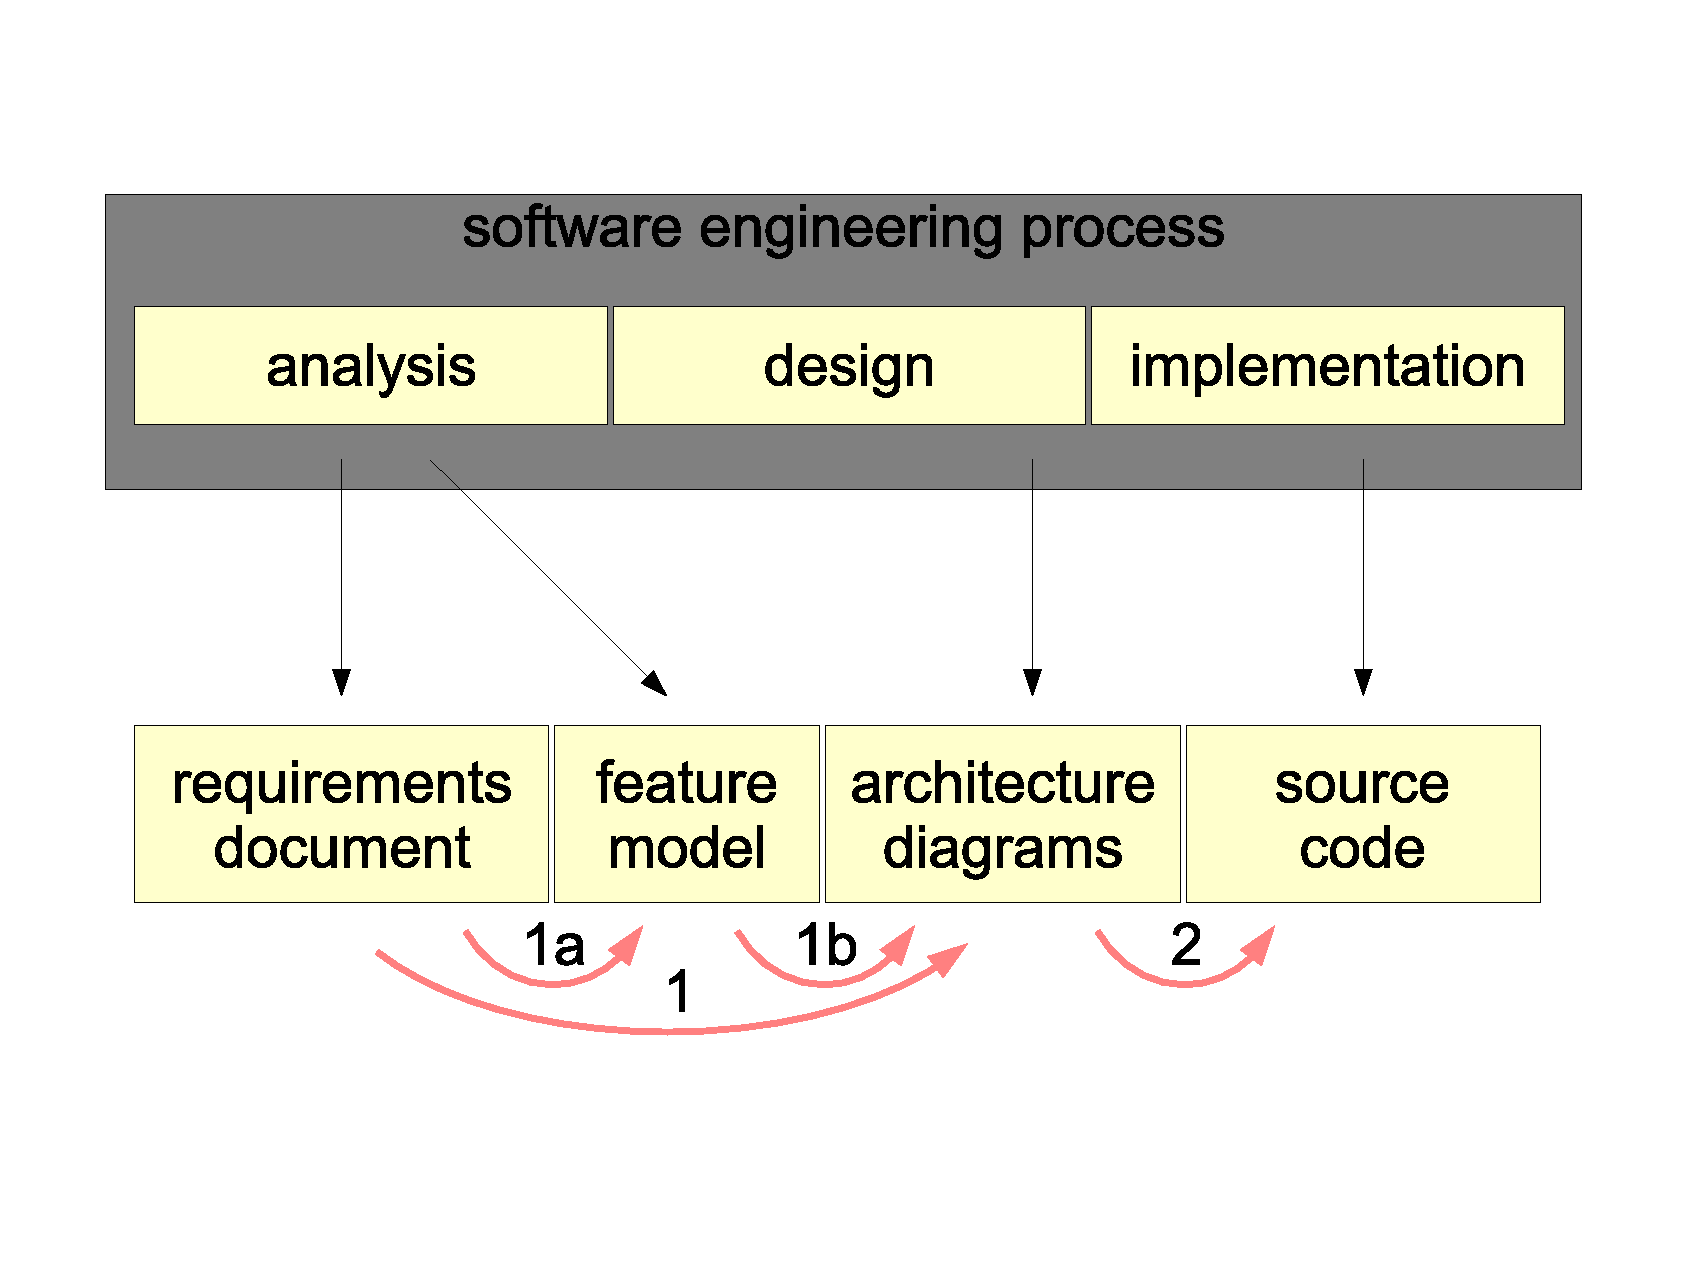
\includegraphics[scale=0.2]{vector/gaps.eps}
        \caption{Abstraction Gaps}
        \label{gaps_figure}
    \end{center}
\end{figure}

Different forms of SEP exist: \emph{Waterfall},\\ \emph{Iterative},
\emph{Extreme Programming} (XP) and \emph{Agile Programming}. But every
project, consciously or not, follows a SEP that sooner-or-later, in one form or
the other, goes through three common phases: \emph{Analysis}, \emph{Design} and
\emph{Implementation}. Each phase creates its own model of what is to be
abstracted in software and it is the differences in exactly these models that
often cause complications.

A previous article \cite{heller2004} mentioned the\\ \emph{Requirements Document},
\emph{Feature Model},\\ \emph{Architecture Diagrams} and \emph{Source Code} as
forms of knowledge abstraction. It also described the following abstraction
gaps (see figure \ref{gaps_figure}) that have to be crossed:

\begin{enumerate}
    \item[1a] Requirements Document -- Feature M.
    \item[1b] Feature Model -- Architecture Diagr.
    \item[2] Architecture Diagrams -- Source Code
\end{enumerate}

By improving the \emph{Traceability} between requirements and the architecture,
feature models (known from system family/ product line engineering) contribute
to minimising gap 1. Together with architecture diagrams, they ease
communication between stakeholders in the SEP, because of their human-readable
form and implementation-independence. But sooner-or-later, also these have to
be transferred into source code, by crossing gap 2.

Bridging or closing these abstraction gaps (sometimes called \emph{Semantic- or
Conceptual Gaps}) is also known as: \textit{achieving higher intentionality}
and remains an unsolved task for software engineering. One aim of the work
described in this article was to contribute to a possible solution, with focus
on \emph{reducing} gap 2, existing between a designed architecture and the
implemented code.

%
% $RCSfile: misleading_tiers.tex,v $
%
% Copyright (c) 2005-2006. Christian Heller. All rights reserved.
%
% Permission is granted to copy, distribute and/or modify this document
% under the terms of the GNU Free Documentation License, Version 1.1 or
% any later version published by the Free Software Foundation; with no
% Invariant Sections, with no Front-Cover Texts and with no Back-Cover
% Texts. A copy of the license is included in the section entitled
% "GNU Free Documentation License".
%
% http://www.cybop.net
% - Cybernetics Oriented Programming -
%
% http://www.resmedicinae.org
% - Information in Medicine -
%
% Version: $Revision: 1.1 $ $Date: 2006-01-03 08:21:45 $ $Author: christian $
% Authors: Christian Heller <christian.heller@tuxtax.de>
%

\subsection{Misleading Tiers}
\label{misleading_tiers_heading}

When distinguishing human- and technical systems, the kinds of
\emph{Communication} are:

\begin{itemize}
    \item[-] Human $\leftrightarrow$ Human
    \item[-] Human $\leftrightarrow$ Computer
    \item[-] Computer $\leftrightarrow$ Computer
\end{itemize}

Each of these relies on different techniques, transport mechanisms, languages
(protocols) and so on. But the general principle after which communication
works, is always the same -- no matter whether technical \emph{Computer}
systems or their biological prototype, the \emph{Human Being}, are considered:
Information is \emph{received}, \emph{stored}, \emph{processed} and \emph{sent}.
Despite these common characteristics, today's \emph{Information Technology}
(IT) environments \cite{hellerkunze} treat communication between a computer
system and a human being differently than that \emph{among} computer systems.

\begin{figure}[ht]
    \begin{center}
        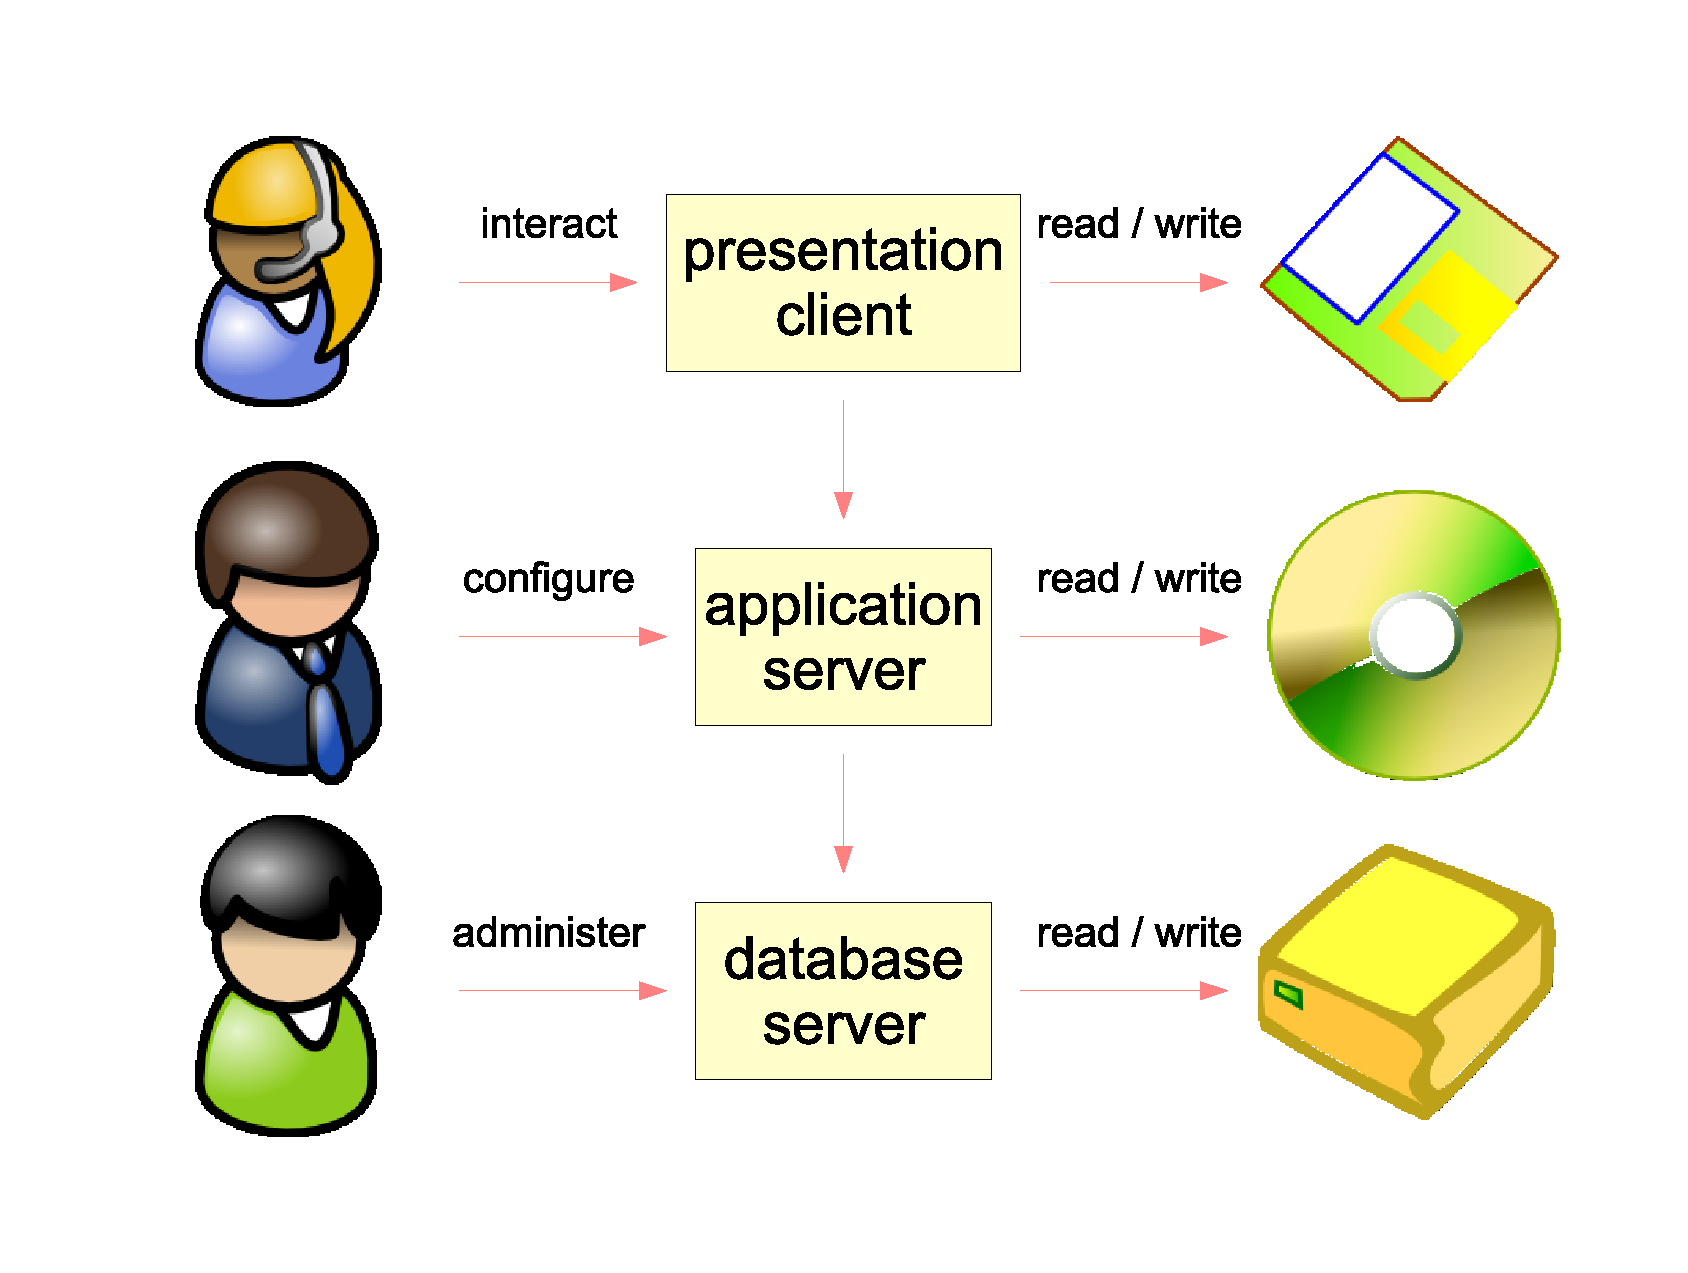
\includegraphics[scale=0.2]{vector/universal.eps}
        \caption{Universal Communication}
        \label{universal_figure}
    \end{center}
\end{figure}

Figure \ref{universal_figure} shows a three-tier environment: tier 1 represents
the \emph{Presentation Layer}; tier 2 stands for the \emph{Application Layer};
tier 3 is the \emph{Database (DB) Layer}. Typical synonyms are, in this order:
\emph{Frontend}, \emph{Business Logic} and \emph{Backend}. The tiers (layers)
serve two needs: connect different locations and share work load (\emph{Scaling}).
However, the split into tiers of that kind raises two illusions:

\begin{enumerate}
    \item \emph{Users only interact with clients}
    \item \emph{Persistent data are stored in DB only}
\end{enumerate}

Many IT architectures, or at least their illustrations, neglect the fact that
in reality \emph{all} systems need a \emph{User Interface} (UI), for at least
being administered by humans, and \emph{almost} all systems, even
\emph{Database Management Systems} (DBMS) themselves, store some of their
persistent data outside a database, for example locally available configuration
information. This is not necessarily a problem for the IT environment as such,
but it is for the internal architecture of software systems. Special solutions
have to deal with frontend (UI framework), business logic (domain patterns) and
backend (data mapping), and often additional mechanisms for local and remote
communication. The serious differences in these design solutions are one root
of well-known problems like multi- directional inter-dependencies between system
parts, that make software difficult to develop and hard to maintain.

One aim of the work described in this article was to investigate possibilities
for a \emph{unification} of communication paradigms, that is high-level design
paradigms rather than low-level protocols, in order to architect software in a
way that allows the computer system it runs on to communicate \emph{universally}.

%
% $RCSfile: modelling_mistakes.tex,v $
%
% Copyright (c) 2005-2006. Christian Heller. All rights reserved.
%
% Permission is granted to copy, distribute and/or modify this document
% under the terms of the GNU Free Documentation License, Version 1.1 or
% any later version published by the Free Software Foundation; with no
% Invariant Sections, with no Front-Cover Texts and with no Back-Cover
% Texts. A copy of the license is included in the section entitled
% "GNU Free Documentation License".
%
% http://www.cybop.net
% - Cybernetics Oriented Programming -
%
% http://www.resmedicinae.org
% - Information in Medicine -
%
% Version: $Revision: 1.1 $ $Date: 2006-01-03 08:21:45 $ $Author: christian $
% Authors: Christian Heller <christian.heller@tuxtax.de>
%

\subsection{Modelling Mistakes}
\label{modelling_mistakes_heading}

Most modern software is not written directly in a machine language but designed
in form of higher-level models instead. These allow to speed up application
development and help avoiding errors. \emph{Object Oriented Programming} (OOP),
for example, uses design concepts like the \emph{Class} owning \emph{Attributes}
and \emph{Methods}. Yet does this kind of modelling create abstractions that
reflect concepts of the real world completely and correctly?

\begin{figure}[ht]
    \begin{center}
        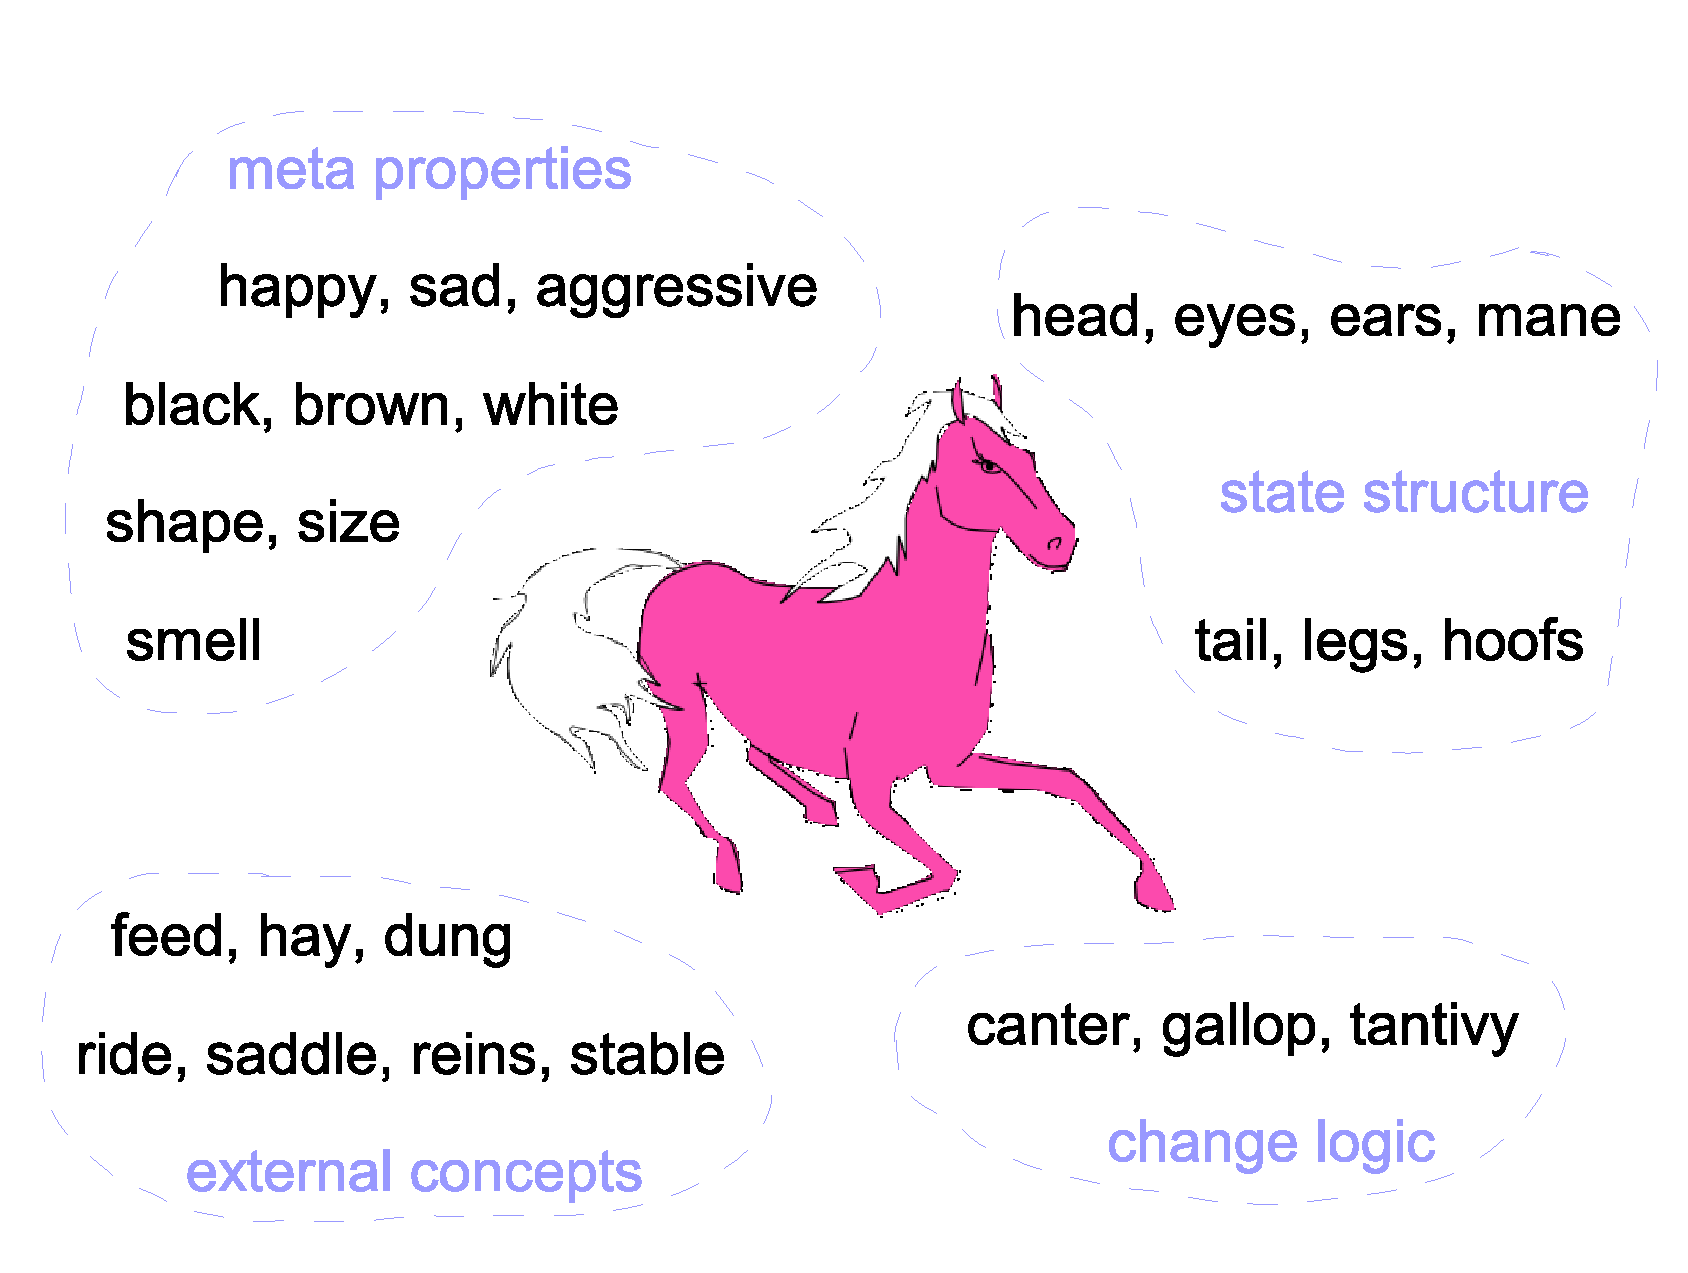
\includegraphics[scale=0.2]{vector/horse.eps}
        \caption{Concept of a Horse}
        \label{horse_figure}
    \end{center}
\end{figure}

The model of a \emph{Horse} shall serve as example to investigate this further.
Figure \ref{horse_figure} shows a number of terms commonly used to describe a
horse. Most importantly, there are structural observations describing the horse
as concept consisting of parts like \emph{Head}, \emph{Legs} or \emph{Hoofs}.
Secondly, there are properties like the horse's \emph{Colour}, \emph{Shape} or
\emph{Size}. Thirdly, there are terms describing a horse's actions like its
\emph{Movement} or \emph{Eating}, that change a horse's position and/ or state.
Finally, there are a number of terms like \emph{Hay} or \emph{Saddle}
associating concepts related to the horse.

One might suggest to model properties like the position, size or colour of a
horse's leg as \emph{Part} of that leg. In fact, this is how classical
programming approaches its solutions. In OOP, one would probably use a class
representing the leg and an attribute standing for the leg's colour. However,
when following the modelling principles of human thinking (see
\cite{heller2004}), this is \emph{not} correct!

It is true that in everyday language, one tends to say \textit{A horse leg
\emph{has a} colour.} Unfortunately, this leads to the wrong assumption that a
leg were made of a colour. But this is not the case. A leg does not
\emph{consist} of a colour in the hierarchical meaning of a whole consisting of
parts. The colour is rather property information \emph{about} the leg. It seems
there is no correct expression in natural (English) language stating the
property of something. The \emph{IS-A} verbalisation is used to express that
the leg belongs to a special category of items, for example: \textit{A leg is a
body element.} The \emph{HAS-A} formulation is used to express that a leg as
whole consists of smaller parts, for example: \textit{A leg has a knee and it
has a hoof.} But which formulation expresses a property? Well, perhaps it would
be best to say: \textit{A leg IS-OF a colour.}

The CYBOP knowledge schema described later in this article distinguishes
structural- from meta information. Actions (like the gallop of a horse) causing
change in the model or its environment are called \emph{Logic} in this work,
since they follow certain rules.


    \newpage{\pagestyle{empty}\cleardoublepage}
    \input{basics}
    \newpage{\pagestyle{empty}\cleardoublepage}
    \input{contribution}
    \newpage{\pagestyle{empty}\cleardoublepage}
    %
% $RCSfile: proof.tex,v $
%
% Copyright (C) 2002-2008. Christian Heller.
%
% Permission is granted to copy, distribute and/or modify this document
% under the terms of the GNU Free Documentation License, Version 1.1 or
% any later version published by the Free Software Foundation; with no
% Invariant Sections, with no Front-Cover Texts and with no Back-Cover
% Texts. A copy of the license is included in the section entitled
% "GNU Free Documentation License".
%
% http://www.cybop.net
% - Cybernetics Oriented Programming -
%
% http://www.resmedicinae.org
% - Information in Medicine -
%
% Version: $Revision: 1.1 $ $Date: 2008-08-19 20:41:08 $ $Author: christian $
% Authors: Christian Heller <christian.heller@tuxtax.de>
%

\part{Proof}
\label{proof_heading}
\newpage{\pagestyle{empty}\cleardoublepage}

%
% $RCSfile: cybernetics_oriented_language.tex,v $
%
% Copyright (C) 2002-2008. Christian Heller.
%
% Permission is granted to copy, distribute and/or modify this document
% under the terms of the GNU Free Documentation License, Version 1.1 or
% any later version published by the Free Software Foundation; with no
% Invariant Sections, with no Front-Cover Texts and with no Back-Cover
% Texts. A copy of the license is included in the section entitled
% "GNU Free Documentation License".
%
% http://www.cybop.net
% - Cybernetics Oriented Programming -
%
% http://www.resmedicinae.org
% - Information in Medicine -
%
% Version: $Revision: 1.1 $ $Date: 2008-08-19 20:41:06 $ $Author: christian $
% Authors: Christian Heller <christian.heller@tuxtax.de>
%

\chapter{Cybernetics Oriented Language}
\label{cybernetics_oriented_language_heading}
\index{Cybernetics Oriented Language}
\index{CYBOL}

\begin{flushright}
    \textsl{The Whole is more than the Sum of its Parts.}\\
    \textsc{Aristotle}
\end{flushright}

Chapter \ref{knowledge_schema_heading} introduced a new model for structuring
knowledge, which chapter \ref{state_and_logic_heading} separated into state-
and logic knowledge. What still has to be given though, is a
\emph{Proof of Operability} for these concepts. The following sections will
therefore define the \emph{Cybernetics Oriented Language} (CYBOL), which
contains all new principles and ideas, as first mentioned in \cite{heller2004}.

%
% $RCSfile: formality.tex,v $
%
% Copyright (C) 2002-2008. Christian Heller.
%
% Permission is granted to copy, distribute and/or modify this document
% under the terms of the GNU Free Documentation License, Version 1.1 or
% any later version published by the Free Software Foundation; with no
% Invariant Sections, with no Front-Cover Texts and with no Back-Cover
% Texts. A copy of the license is included in the section entitled
% "GNU Free Documentation License".
%
% http://www.cybop.net
% - Cybernetics Oriented Programming -
%
% http://www.resmedicinae.org
% - Information in Medicine -
%
% Version: $Revision: 1.1 $ $Date: 2008-08-19 20:41:06 $ $Author: christian $
% Authors: Christian Heller <christian.heller@tuxtax.de>
%

\section{Formality}
\label{formality_heading}
\index{Formality}
\index{Informal Language}
\index{Semi-Formal Diagrams}
\index{Formal Programming Language}
\index{Machine Language}
\index{Knowledge Modelling Language}

Abstract models can be described in different ways, for example \cite{philippow}:

\begin{itemize}
    \item[-] \emph{informally} by natural language
    \item[-] \emph{semi-formally} by diagrams
    \item[-] \emph{formally} by a programming language
\end{itemize}

The use of a programming language eases model abstraction for human programmers.
Special tools exist that break down models given in form of programming language
code into their binary form, into sequences of \emph{0} and \emph{1}. These
sequences are called \emph{Machine Language} because they are understood by
computers.

Classical programming languages have the linguistic means to express high-level
\emph{Knowledge} as well as low-level \emph{System Control} operations, such as
those for \emph{input/ output} (i/o), necessary for communication. The use of
such languages inevitably leads to a mess in program code because knowledge and
system control are mixed up. Inflexible, overly complex systems with numerous
interdependencies are the result. Part \ref{basics_heading} of this work
criticised some of the weak points of traditional programming language concepts.

This work makes the necessary split: Knowledge gets \emph{separated} from
system control. Chapter \ref{statics_and_dynamics_heading} already discussed
this separation giving manifold examples, taken from several sciences. The CYBOL
language being described in the next sections is just another form of storing
knowledge. It can therefore also be called a \emph{Knowledge Modelling Language}.
Any other low-level system control functionality belongs to the
\emph{Cybernetics Oriented Interpreter} (CYBOI), which gets introduced in the
later chapter \ref{cybernetics_oriented_interpreter_heading}.

%
% $RCSfile: definition.tex,v $
%
% Copyright (c) 2002-2007. Christian Heller. All rights reserved.
%
% Permission is granted to copy, distribute and/or modify this document
% under the terms of the GNU Free Documentation License, Version 1.1 or
% any later version published by the Free Software Foundation; with no
% Invariant Sections, with no Front-Cover Texts and with no Back-Cover
% Texts. A copy of the license is included in the section entitled
% "GNU Free Documentation License".
%
% http://www.cybop.net
% - Cybernetics Oriented Programming -
%
% Version: $Revision: 1.2 $ $Date: 2007-08-01 13:59:00 $ $Author: christian $
% Authors: Christian Heller <christian.heller@tuxtax.de>
%

\chapter{Definition}
\label{definition_heading}
\index{Definition}
\index{Whole-Part Hierarchy}
\index{Meta Data Hierarchy}
\index{Extensible Markup Language}
\index{XML}

This chapter defines the \emph{Syntax}, \emph{Vocabulary} and \emph{Semantics}
of the CYBOL language.

As already mentioned in chapter \ref{introduction_heading}, CYBOL is based upon
\emph{two} kinds of hierarchies. One of them is representing \emph{Whole-Part}
relations (such as a graphical window consisting of a menu bar) and the other
the \emph{Meta Data} which a whole keeps about its parts (such as the size or
colour of the menu bar). More details and the philosophical background are
described in \cite{cybopbook}. The syntax and semantics of CYBOL as new
language must be rich enough to express abstract knowledge models using this
kind of double hierarchy.

\input{syntax}
\input{vocabulary}
\input{semantics}

%
% $RCSfile: constructs.tex,v $
%
% Copyright (C) 2002-2008. Christian Heller.
%
% Permission is granted to copy, distribute and/or modify this document
% under the terms of the GNU Free Documentation License, Version 1.1 or
% any later version published by the Free Software Foundation; with no
% Invariant Sections, with no Front-Cover Texts and with no Back-Cover
% Texts. A copy of the license is included in the section entitled
% "GNU Free Documentation License".
%
% http://www.cybop.net
% - Cybernetics Oriented Programming -
%
% http://www.resmedicinae.org
% - Information in Medicine -
%
% Version: $Revision: 1.1 $ $Date: 2008-08-19 20:41:06 $ $Author: christian $
% Authors: Christian Heller <christian.heller@tuxtax.de>
%

\section{Constructs}
\label{constructs_heading}
\index{CYBOL Constructs}

After having defined the CYBOL language in the previous section, the following
examples can demonstrate how the language's constructs may be used in practice.
Attention is also payed to how control structures of classical programming
languages (compare section \ref{structured_and_procedural_programming_heading})
may be implemented in CYBOL. Additionally, this section discusses how
inheritance, containers and software patterns were considered in the design of
CYBOL.

\input{state_examples}
\input{logic_examples}
\input{special_examples}
\input{inheritance_as_property}
\input{container_mapping}
\input{hidden_patterns}

%
% $RCSfile: comparison.tex,v $
%
% Copyright (c) 2002-2007. Christian Heller. All rights reserved.
%
% Permission is granted to copy, distribute and/or modify this document
% under the terms of the GNU Free Documentation License, Version 1.1 or
% any later version published by the Free Software Foundation; with no
% Invariant Sections, with no Front-Cover Texts and with no Back-Cover
% Texts. A copy of the license is included in the section entitled
% "GNU Free Documentation License".
%
% http://www.cybop.net
% - Cybernetics Oriented Programming -
%
% Version: $Revision: 1.1 $ $Date: 2007-07-17 20:02:36 $ $Author: christian $
% Authors: Christian Heller <christian.heller@tuxtax.de>
%

\section{Comparison}
\label{comparison_heading}
\index{Comparison}

\input{compare}

%
% $RCSfile: tool_support.tex,v $
%
% Copyright (C) 2002-2008. Christian Heller.
%
% Permission is granted to copy, distribute and/or modify this document
% under the terms of the GNU Free Documentation License, Version 1.1 or
% any later version published by the Free Software Foundation; with no
% Invariant Sections, with no Front-Cover Texts and with no Back-Cover
% Texts. A copy of the license is included in the section entitled
% "GNU Free Documentation License".
%
% http://www.cybop.net
% - Cybernetics Oriented Programming -
%
% http://www.resmedicinae.org
% - Information in Medicine -
%
% Version: $Revision: 1.1 $ $Date: 2008-08-19 20:41:09 $ $Author: christian $
% Authors: Christian Heller <christian.heller@tuxtax.de>
%

\section{Tool Support}
\label{tool_support_heading}
\index{CYBOL Tool Support}

When proposing a new theory of computing, or a new programming language, it is
common to provide a suitable \emph{Integrated Development Environment} (IDE)
supporting the application of that theory or language. If not the tools
themselves, a recommendation for how they may look like should be given at
least. This is what the following sections try to achieve.

\input{template_editor}
\input{knowledge_designer}
\input{model_viewer}

To what concerns the usage of existing UML tools for modelling CYBOL
applications, it has to be said that they are most likely not able to support
CYBOP models, nor can they be easily adapted. Even though the diagram
specifications may be similar, the underlying programming principles and model
repositories are just too different. It might be possible, however, to create
interfaces partly translating CYBOL-encoded (XML) models into UML models,
possibly using the \emph{XML Metadata Interchange} (XMI) standard or the like.
It will presumably be easier to translate CYBOL- into UML models, than vice
versa, because CYBOL is very expressive. While CYBOL knowledge templates
distinguish between whole-part- and meta elements, for example, UML models do
not. Another point is that CYBOL holds state- and logic knowledge in separate
templates, that would have to be merged into common classes when being
translated into UML. But the investigation and evaluation of further details
concerning the tool support is left for future works.


\newpage{\pagestyle{empty}\cleardoublepage}
%
% $RCSfile: cybernetics_oriented_interpreter.tex,v $
%
% Copyright (c) 2001-2004. Christian Heller. All rights reserved.
%
% No copying, altering, distribution or any other actions concerning this
% document, except after explicit permission by the author!
% At some later point in time, this document is planned to be put under
% the GNU FDL license. For now, _everything_ is _restricted_ by the author.
%
% http://www.cybop.net
% - Cybernetics Oriented Programming -
%
% http://www.resmedicinae.org
% - Information in Medicine -
%
% @author Christian Heller <christian.heller@tuxtax.de>
%

\subsection{Cybernetics Oriented Interpreter}
\label{cybernetics_oriented_interpreter_heading}

The CYBOL language described in section \ref{cybernetics_oriented_language_heading}
is just another form of storing knowledge. It can therefore also be called a
\emph{Knowledge Modelling Language}.

\begin{figure}[ht]
    \begin{center}
        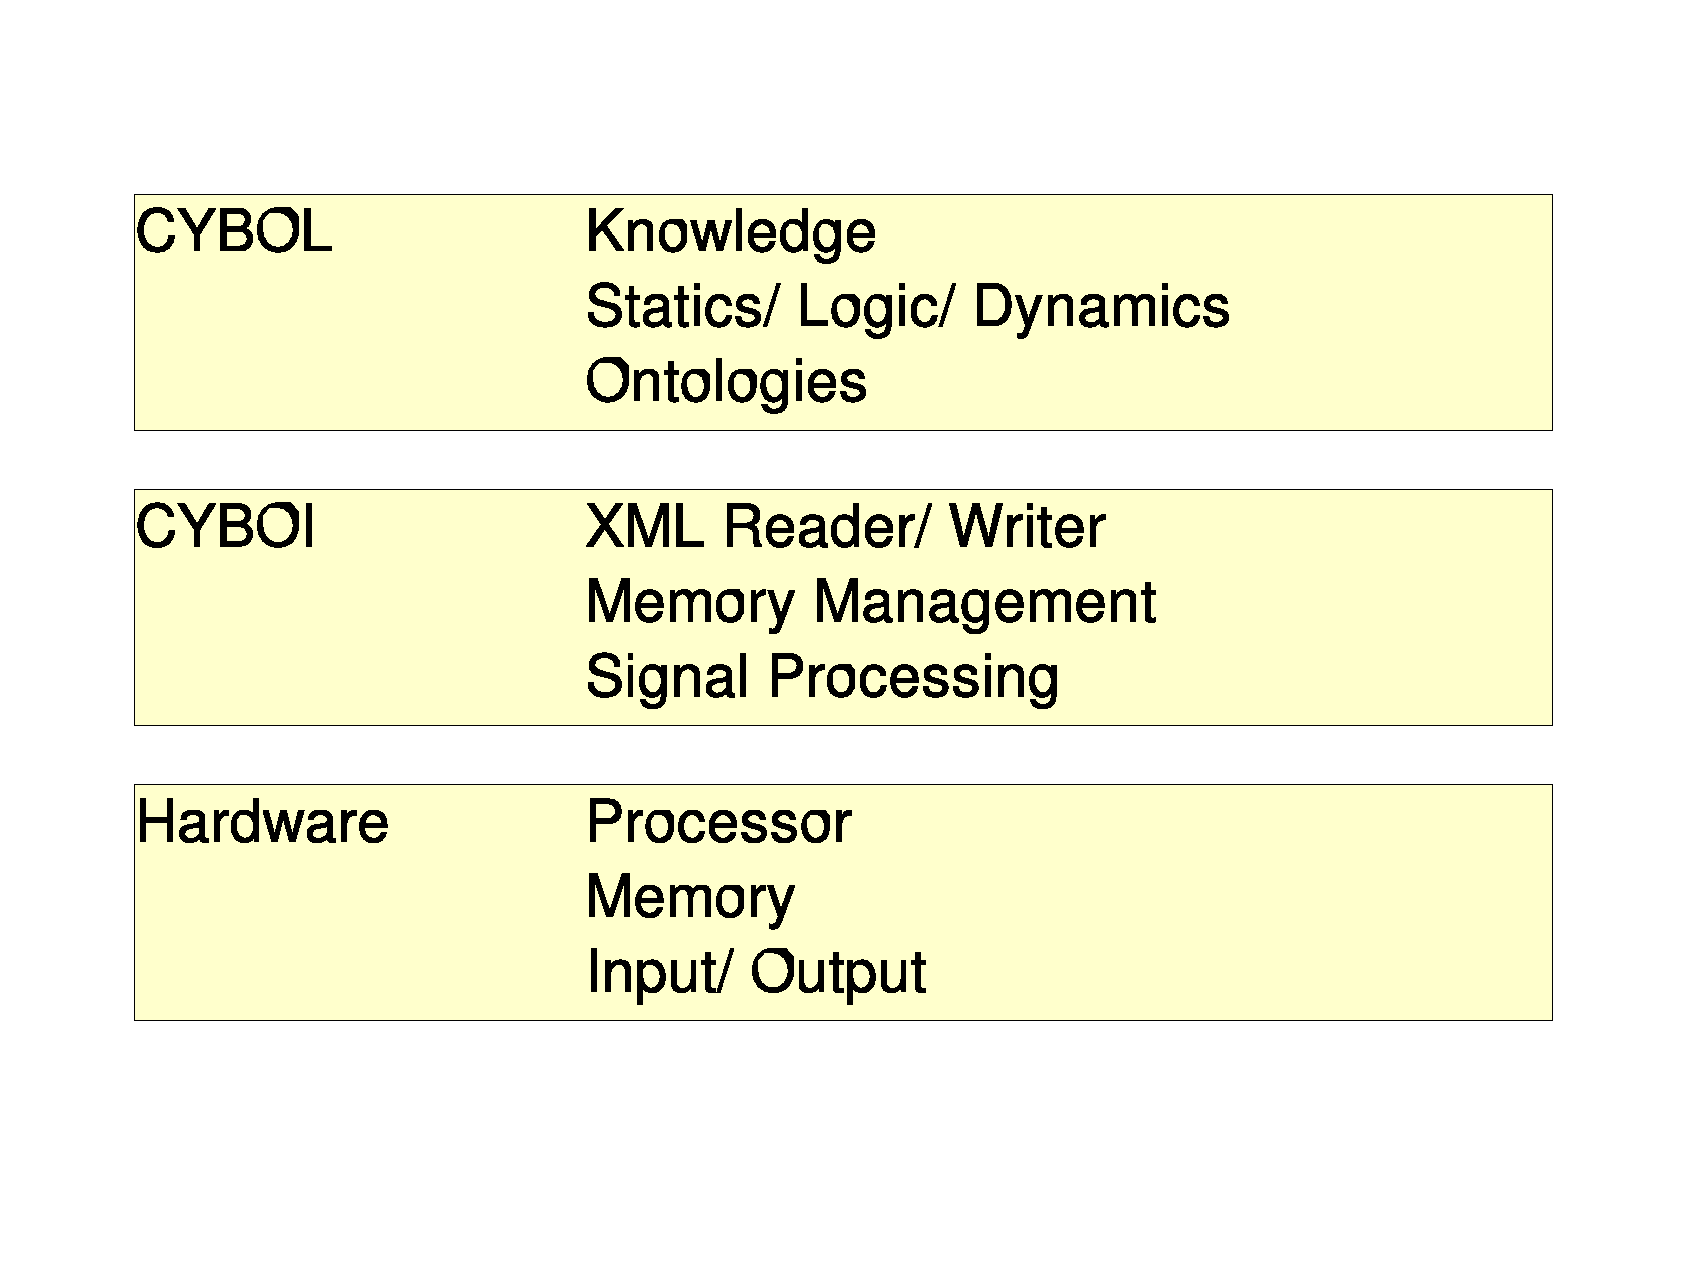
\includegraphics[scale=0.3]{vector/hardware_connection.eps}
        \caption{CYBOI as Interface between CYBOL and Hardware}
        \label{hardware_connection_figure}
    \end{center}
\end{figure}

When CYBOL files contain the knowledge that
defines a system, a counterpart is needed to execute that system on computer
hardware. The \emph{Cybernetics Oriented Interpreter} (CYBOI) is able to handle
this task (figure \ref{hardware_connection_figure}).
CYBOI is written in the C programming language and currently supports the
\emph{Linux} \emph{Operating System} (OS) only. It represents, so to say, the
interface between operating instructions of the computer hardware and system
models defined in CYBOL.

CYBOI is responsible for managing any kind of hardware communication, that is
input, output, memory access and processor instruction calls. CYBOI Signals can
be assigned priorities, a language (protocol) to communicate with other systems
and they are processed by one single loop (figure \ref{cyboi_figure}). Also,
there is only one single container structure which CYBOI uses to dynamically
store knowledge. It such avoids the known problems with container inheritance
\cite{javaiaq}. Following \emph{Euclidian Geometry}, multi-dimensional
\emph{Models} consist of maps; two-dimensional \emph{Maps} consist of arrays;
one-dimensional \emph{Arrays} represent and manage an area in the computer memory.

\begin{figure}[ht]
    \begin{center}
        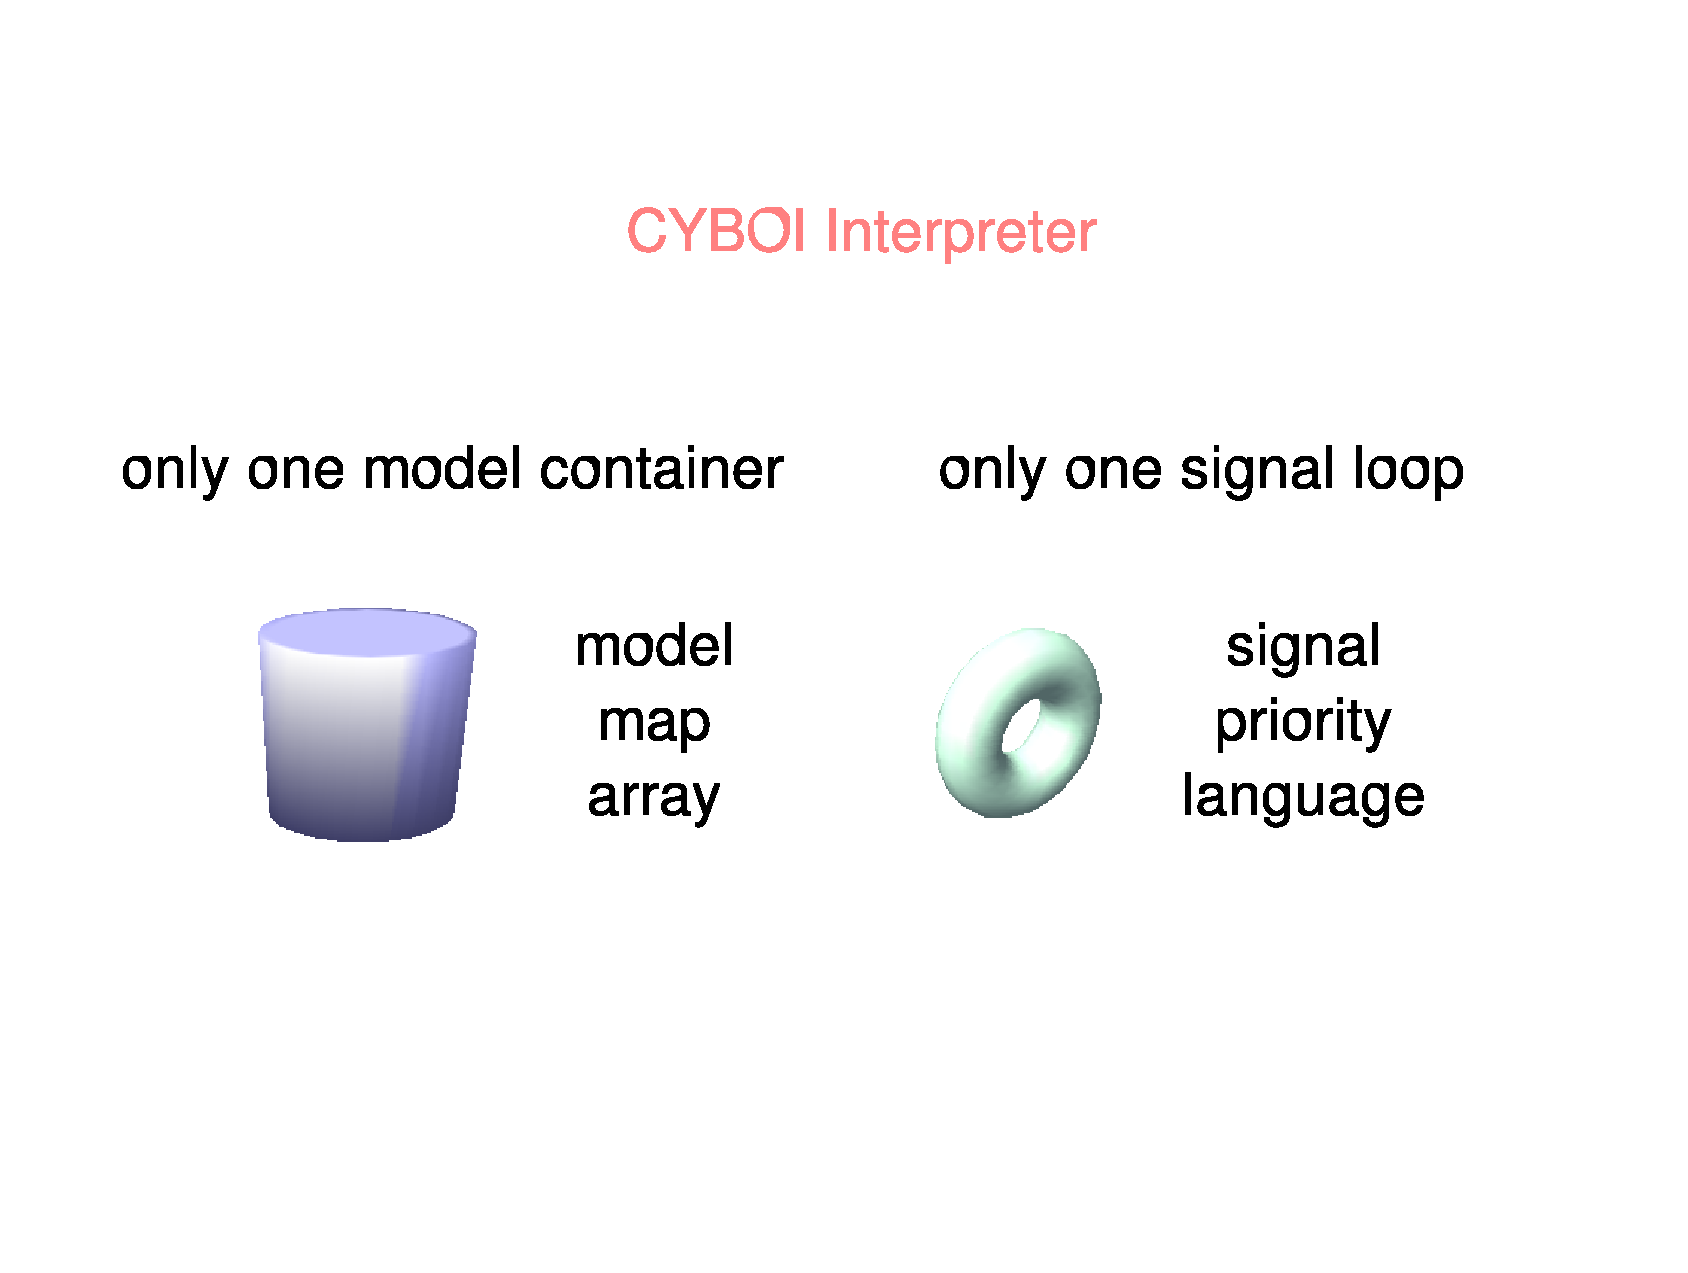
\includegraphics[scale=0.3]{vector/cyboi.eps}
        \caption{CYBOI Model Container and Signal Loop}
        \label{cyboi_figure}
    \end{center}
\end{figure}

The more hardware driving functionality CYBOI implements, the more it develops
towards an operating system -- with one difference to current OS: It is free of
any configuration information but knows how to \emph{handle} knowledge.

\newpage{\pagestyle{empty}\cleardoublepage}
%
% $RCSfile: res_medicinae.tex,v $
%
% Copyright (C) 2002-2008. Christian Heller.
%
% Permission is granted to copy, distribute and/or modify this document
% under the terms of the GNU Free Documentation License, Version 1.1 or
% any later version published by the Free Software Foundation; with no
% Invariant Sections, with no Front-Cover Texts and with no Back-Cover
% Texts. A copy of the license is included in the section entitled
% "GNU Free Documentation License".
%
% http://www.cybop.net
% - Cybernetics Oriented Programming -
%
% http://www.resmedicinae.org
% - Information in Medicine -
%
% Version: $Revision: 1.1 $ $Date: 2008-08-19 20:41:08 $ $Author: christian $
% Authors: Christian Heller <christian.heller@tuxtax.de>
%

\chapter{Res Medicinae}
\label{res_medicinae_heading}
\index{Res Medicinae Application Prototype}

\begin{flushright}
    \textsl{
        No Road can ever be too long,\\
        side-by-side with a good Friend.
    }\\
    \textsc{Unknown Author}
\end{flushright}

The first two chapters (\ref{cybernetics_oriented_language_heading} and
\ref{cybernetics_oriented_interpreter_heading}) of part \ref{proof_heading} of
this work defined the CYBOL language and its corresponding interpreter CYBOI.
Since a theory is worth more if it can be proven in practice, this chapter will
describe an effort trying to apply both to create an application system named
\emph{Res Medicinae} \cite{resmedicinae} (Latin for \emph{Matter of Medicine}).

%
% $RCSfile: project.tex,v $
%
% Copyright (C) 2002-2008. Christian Heller.
%
% Permission is granted to copy, distribute and/or modify this document
% under the terms of the GNU Free Documentation License, Version 1.1 or
% any later version published by the Free Software Foundation; with no
% Invariant Sections, with no Front-Cover Texts and with no Back-Cover
% Texts. A copy of the license is included in the section entitled
% "GNU Free Documentation License".
%
% http://www.cybop.net
% - Cybernetics Oriented Programming -
%
% http://www.resmedicinae.org
% - Information in Medicine -
%
% Version: $Revision: 1.1 $ $Date: 2008-08-19 20:41:08 $ $Author: christian $
% Authors: Christian Heller <christian.heller@tuxtax.de>
%

\section{Project}
\label{project_heading}
\index{Res Medicinae Project}
\index{Hospital Information System}
\index{HIS}
\index{Practice Management System}
\index{PMS}
\index{Electronic Health Record}
\index{EHR}

The -- somewhat idealistic -- aim was initially to create the prototype of a
\emph{Hospital Information System} (HIS). Due to the clearly too high-set aims,
this was later revised so that the focus of the prototype became a standard
\emph{Practice Management System} (PMS) with an \emph{Electronic Health Record}
(EHR) as its core. Several technology changes during the progress of this work
and the lack in time required to also revise this aim, so that now the final
prototype consists of just the (rudimentary) address management module of the
planned EHR application. It is written in CYBOL and executable by CYBOI.

The following sections describe the project background of \emph{Res Medicinae}.

\input{free_and_open_source_software}
\input{portals_and_services}
\input{tools}
\input{contributors}

%
% $RCSfile: analysis.tex,v $
%
% Copyright (C) 2002-2008. Christian Heller.
%
% Permission is granted to copy, distribute and/or modify this document
% under the terms of the GNU Free Documentation License, Version 1.1 or
% any later version published by the Free Software Foundation; with no
% Invariant Sections, with no Front-Cover Texts and with no Back-Cover
% Texts. A copy of the license is included in the section entitled
% "GNU Free Documentation License".
%
% http://www.cybop.net
% - Cybernetics Oriented Programming -
%
% http://www.resmedicinae.org
% - Information in Medicine -
%
% Version: $Revision: 1.1 $ $Date: 2008-08-19 20:41:05 $ $Author: christian $
% Authors: Christian Heller <christian.heller@tuxtax.de>
%

\section{Analysis}
\label{analysis_heading}
\index{Res Medicinae Requirements Analysis}
\index{Software Engineering Process}
\index{SEP}
\index{Electronic Health Record}
\index{EHR}

Abiding by the standard \emph{Software Engineering Process} (SEP) (chapter
\ref{software_engineering_process_heading}), a \emph{Requirements Analysis}
stood as first activity for the development of \emph{Res Medicinae}. The
following sections will give a brief overview of some requirements and current
modelling trends, concerning the \emph{Electronic Health Record} (EHR). They do
\emph{not} try to replace more comprehensive works written on the subject.

\input{requirements_document}
\input{ehr_and_co}
\input{episode_based}
\input{evidence_based}
\input{continuity_of_care}
\input{core_model}

\newpage
%
% $RCSfile: standards.tex,v $
%
% Copyright (C) 2002-2008. Christian Heller.
%
% Permission is granted to copy, distribute and/or modify this document
% under the terms of the GNU Free Documentation License, Version 1.1 or
% any later version published by the Free Software Foundation; with no
% Invariant Sections, with no Front-Cover Texts and with no Back-Cover
% Texts. A copy of the license is included in the section entitled
% "GNU Free Documentation License".
%
% http://www.cybop.net
% - Cybernetics Oriented Programming -
%
% http://www.resmedicinae.org
% - Information in Medicine -
%
% Version: $Revision: 1.1 $ $Date: 2008-08-19 20:41:09 $ $Author: christian $
% Authors: Christian Heller <christian.heller@tuxtax.de>
%

\section{Standards}
\label{standards_heading}
\index{Medical Informatics Standards}

In a further thought, current standards of medical informatics had to be
considered for the development of \emph{Res Medicinae} application modules.
There exists a whole plethora of (partly \emph{de facto}) standards -- far too
many to discuss here. The following sections will give a brief overview of only
a few standards which are potentially important for EHR development.

\input{overview}
\input{record_modelling}
\input{messaging_and_communication}
\input{terminology_systems}
\input{further_standards}
\input{standards_development}
\input{implication}

%
% $RCSfile: realisation.tex,v $
%
% Copyright (C) 2002-2008. Christian Heller.
%
% Permission is granted to copy, distribute and/or modify this document
% under the terms of the GNU Free Documentation License, Version 1.1 or
% any later version published by the Free Software Foundation; with no
% Invariant Sections, with no Front-Cover Texts and with no Back-Cover
% Texts. A copy of the license is included in the section entitled
% "GNU Free Documentation License".
%
% http://www.cybop.net
% - Cybernetics Oriented Programming -
%
% http://www.resmedicinae.org
% - Information in Medicine -
%
% Version: $Revision: 1.1 $ $Date: 2008-08-19 20:41:08 $ $Author: christian $
% Authors: Christian Heller <christian.heller@tuxtax.de>
%

\section{Realisation}
\label{realisation_heading}
\index{Res Medicinae Steps of Realisation}

Having analysed the domain of healthcare and having investigated corresponding
standards, actual design solutions that have been tried out in the course of
this work, by implementing them in software source code, can be described in
the following sections.

\input{student_works}
\input{first_trial}
\input{knowledge_separation}
\input{reimplementation}
\input{module_modelling}



    \newpage{\pagestyle{empty}\cleardoublepage}
    \input{completion}
\end{document}
